%% Seminar deck: Supply, habitat and the price of liquidity (BIR, 2026)
%% 14 slides, yieldcartography house theme, academic-seminar register.
%% Built from the published BIR version (liquidity_paper_v8).
\documentclass[aspectratio=169,11pt]{beamer}
\usepackage{beamerthemeyc}
\renewcommand{\deckfootertitle}{Dec (2026) · Supply, habitat and the price of liquidity · Borsa Istanbul Review}

\begin{document}

% 1 ---------------------------------------------------------------------------
\begin{frame}[plain]
  \vspace{2mm}
  {\ttfamily\scriptsize\color{ycmuted}SEMINAR DECK · YIELDCARTOGRAPHY.COM}\\[-0.3em]
  {\color{ycrule}\rule{\textwidth}{0.5pt}}
  \vspace{4mm}

  {\fontsize{19}{23}\selectfont\bfseries\color{ycink}Supply, habitat and the price of liquidity\\in less-liquid sovereign bond markets.\par}
  \vspace{2mm}
  {\normalsize\color{ycmuted}Evidence from Poland.\par}
  \vspace{6mm}
  {\small\bfseries Marcin Dec\par}
  {\footnotesize\color{ycmuted}Kozminski University \& FAME|GRAPE, Warsaw\par}
  \vspace{3mm}
  {\ttfamily\scriptsize\color{ycaccent}Borsa Istanbul Review, 2026 · open access · doi:10.1016/j.bir.2026.100904\par}
  \vfill
  \raisebox{-1mm}{
\includegraphics[height=6mm]{kozminski_logo.png}}\hspace{5mm}
  \raisebox{-1mm}{
\includegraphics[height=6mm]{grape_logo.png}}\hspace{5mm}
  \raisebox{-1mm}{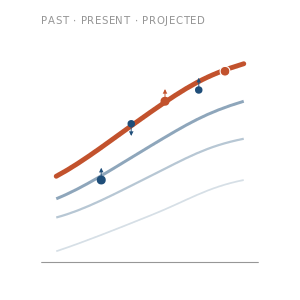
\includegraphics[height=6mm]{yc_logo.png}}
  \hfill{\ttfamily\scriptsize\color{ycmuted}NCN Preludium UMO-2020/37/N/HS4/02202}
\end{frame}

% 2 ---------------------------------------------------------------------------
\begin{frame}{Motivation and contribution}
  \kicker{Research question}
  \begin{itemize}
    \item The low-frequency liquidity-estimator literature is calibrated on
          deep markets; the supply-and-habitat literature
          (Greenwood--Vayanos 2014, Vayanos--Vila 2021) is estimated almost
          exclusively on US Treasuries. Neither has been taken seriously to the
          middle tier of sovereign curves.
    \item This paper treats liquidity as the \alert{dependent variable}:
          what prices into bond-level spreads, into the segment-level supply
          channel, and into the aggregate term premium.
    \item Contribution: a bond-level and segment-level liquidity panel for the
          Polish sovereign curve over 2005--2026, five hypotheses spanning
          issue size, supply stocks, holder structure, monetary events and the
          primary-auction cycle, and a supply-block regression of the price of
          liquidity.
  \end{itemize}
\end{frame}

% 3 ---------------------------------------------------------------------------
\begin{frame}{Setting: the less-liquid market (LLM) cohort}
  \kicker{Institutional environment}
  \begin{itemize}
    \item Middle tier of sovereign curves: liquidity is priced by every dealer,
          yet tick-data estimators built for the deepest curves do not transfer.
          Daily venue fixings and monthly turnover are the highest-frequency
          public record, which dictates the low-frequency estimator set.
    \item Poland is arguably the best-instrumented cohort member: daily
          BondSpot fixings with quoted bid and ask, Ministry of Finance
          holdings by investor class, and a regulated venue with published
          quoting obligations (Annex~G caps).
    \item Comparable markets: Brazil, Chile, Czechia, Hungary, India,
          Indonesia, Israel, Korea, Malaysia, Mexico, Singapore, South Africa,
          Thailand, T\"urkiye.
  \end{itemize}
\end{frame}

% 4 ---------------------------------------------------------------------------
\begin{frame}{Hypotheses}
  \kicker{Testable predictions and expected signs}
  \small
  \begin{itemize}
    \item \textbf{H1 (issue size).} Outstanding amount enters negatively in all
          bond-level liquidity measures.
    \item \textbf{H2 (stocks versus flow).} Segment liquidity responds to stock
          variables (segment stock, residual-maturity concentration), not to
          monthly gross issuance flow.
    \item \textbf{H3 (holder structure).} The post-2019 foreign buy-side
          retreat loads on volume-scaled measures (Amihud) but not on the
          venue-capped quoted spread.
    \item \textbf{H4 (monetary transmission).} The liquidity response to MPC
          rate-change days differs pre- versus post-COVID.
    \item \textbf{H5 (auction cycle).} Primary Dealers absorb auctions at a
          concession; secondary yields revert over the following business week,
          increasing in maturity (inventory risk premium).
  \end{itemize}
\end{frame}

% 4a --------------------------------------------------------------------------
\begin{frame}{Liquidity measures}
  \kicker{Low-frequency estimators on daily fixings}
  \small For bond $i$ in month $t$, from daily closing fixings (price $p$, bid
  $b$, ask $a$, turnover $V$, modified duration $MD$):
  \[ BAS_{it} \;=\; 10^{4}\,\overline{\left(\frac{|a-b|}{p\cdot MD}\right)},
     \qquad
     Amihud_{it} \;=\; \overline{\left(\frac{|r_d|}{V_d}\right)},
     \qquad
     Roll_{it} \;=\; 2\sqrt{-\widehat{\mathrm{Cov}}(\Delta p_d,\Delta p_{d-1})} \]
  \begin{itemize}
    \item Duration scaling converts the quoted price spread into a
          yield-equivalent object, comparable across maturities.
    \item Completed by the Bao--Pan--Wang $\gamma$, the Corwin--Schultz
          high-low estimator, the zero-trading-days share, and an equal-weight
          composite $z$-score of the standardised measures.
  \end{itemize}
\end{frame}

% 4b --------------------------------------------------------------------------
\begin{frame}{Estimating equations}
  \kicker{Three layers}
  \small Bond-month panel (H1--H3), bond fixed effects, Driscoll--Kraay SE:
  \[ L_{it} \;=\; \alpha_i + \beta' X_{it} + \gamma' M_t + \varepsilon_{it} \]
  Aggregate monthly supply block (Result 4), Newey--West SE:
  \[ TP_t^{(\tau)} \;=\; \alpha + \beta_D\, Debt_t + \beta_F\, Foreign_t
     + \beta_N\, NBP_t + \beta_G\, \tfrac{Debt_t}{GDP_t}
     + \delta' M_t + u_t \]
  Auction event study (H5), normalised yield path by segment $s$:
  \[ \Delta y_{s,k} \;=\; y_{s,\,t_e+k} - y_{s,\,t_e},
     \qquad k \in [-5,\,+10] \text{ business days} \]
\end{frame}

% 5 ---------------------------------------------------------------------------
\begin{frame}{Result 1: issue size (H1)}
  \kicker{Bond-month panel, bond FE, Driscoll-Kraay SE}
  \bignum{$-3.5$ bp}{coefficient on log(outstanding) for the quoted spread in
  the bond-month panel with bond fixed effects and Driscoll--Kraay standard
  errors, $p<0.01$. Same sign and significance on the composite $z$-score and
  on the zero-trading-days share.}
  \vspace{1mm}
  \begin{center}\small\color{ycmuted}
  Robust to macro and regime controls, consistent across all six
  low-frequency estimators.
  \end{center}
\end{frame}

% 6 ---------------------------------------------------------------------------
\begin{frame}{Result 2: supply operates through stocks, not flow (H2)}
  \kicker{Segment-month panel, segment FE, Driscoll-Kraay SE}
  \begin{itemize}
    \item Monthly gross issuance is insignificant for segment liquidity once
          stock variables enter the specification.
    \item Trailing twelve-month issuance and log segment stock load
          monotonically; the residual-maturity concentration share loads
          positively on Amihud and on the zero-trading-days share.
    \item Interpretation: the level and the maturity composition of the
          outstanding stock, not the issuance calendar, are the supply margins
          priced into liquidity.
  \end{itemize}
\end{frame}

% 7 ---------------------------------------------------------------------------
\begin{frame}{Result 3: the quote cap separates BAS from Amihud (H3)}
  \kicker{Identification from the venue rulebook}
  \small The foreign buy-side share of zloty-denominated sovereign debt fell
  from ${\sim}33\%$ to under $15\%$ over 2019--2024. The two estimator families
  respond asymmetrically:
  \vspace{3mm}
  \begin{center}
  \begin{tikzpicture}[x=1cm,y=1cm]
    \node[anchor=west,font=\small\bfseries,text=ycink] at (0,2.35) {Quoted spread (BAS)};
    \fill[ycrule] (0,1.75) rectangle (3.4,2.10);
    \node[anchor=west,font=\scriptsize\itshape,text=ycmuted] at (0,1.45)
      {bounded by the Annex G maximum-spread obligations (30--90 ticks)};
    \node[anchor=west,font=\small\bfseries,text=ycink] at (0,0.60) {Amihud price impact};
    \fill[ycsalmon] (0,0.00) rectangle (10.6,0.35);
    \node[anchor=west,font=\scriptsize\itshape,text=ycmuted] at (0,-0.32)
      {unbounded: $+0.29^{***}$ on the foreign share};
  \end{tikzpicture}
  \end{center}
  \vspace{1mm}
  \small\color{ycmuted} Under a binding quote cap, quote-based and volume-scaled
  estimators identify different objects; treating them as substitutes discards
  the identifying variation.
\end{frame}

% 8 ---------------------------------------------------------------------------
\begin{frame}{Result 4: the supply gradient on the term premium}
  \kicker{Monthly time series, Newey-West SE, Andrews bandwidth}
  \small Coefficient on the total State Treasury debt level (per $+100$ bn PLN)
  in monthly regressions of ACM term premia on the supply block and macro
  controls, $n=167$:
  \begin{center}
  \begin{tikzpicture}[x=1.35cm,y=0.095cm]
    \foreach \y in {0,5,10,15,20,25} \draw[ycrule,line width=0.4pt] (0,\y) -- (9,\y);
    \draw[ycmuted,line width=0.5pt] (0,0) -- (9,0);
    \foreach \y in {0,10,20} \node[left=2pt,font=\scriptsize,text=ycmuted] at (0,\y) {\y};
    \fill[ycrule]   (0.8,0) rectangle (2.3,6);
    \node[above,font=\scriptsize\bfseries,text=ycink] at (1.55,6) {+6};
    \node[below,font=\scriptsize,text=ycmuted] at (1.55,-0.5) {2Y};
    \fill[ycaccent!60] (3.7,0) rectangle (5.2,20);
    \node[above,font=\scriptsize\bfseries,text=ycink] at (4.45,20) {+20***};
    \node[below,font=\scriptsize,text=ycmuted] at (4.45,-0.5) {5Y};
    \fill[ycaccent] (6.6,0) rectangle (8.1,23);
    \node[above,font=\scriptsize\bfseries,text=ycink] at (7.35,23) {+23***};
    \node[below,font=\scriptsize,text=ycmuted] at (7.35,-0.5) {10Y};
    \node[right,font=\tiny\itshape,text=ycmuted,rotate=90,anchor=west] at (-0.85,2) {bp per +100 bn PLN};
  \end{tikzpicture}
  \end{center}
  \footnotesize\color{ycmuted} The supply block is jointly significant at 1\%
  for all term-premium maturities ($F$ between 4.3 and 9.5) and insignificant
  for the venue-capped aggregate BAS ($F=0.65$). The tenor-increasing gradient
  is the preferred-habitat signature of Vayanos--Vila (2021), not a uniform
  additive premium. Debt-to-GDP adds ${\sim}+8$ bp at 10Y per pp.
\end{frame}

% 9 ---------------------------------------------------------------------------
\begin{frame}{Result 5: a mark-to-market counterfactual}
  \kicker{Three-curve present-value scenario}
  \small The outstanding fixed-cash-flow universe (951 bn PLN face) is repriced
  under (A) the contemporaneous NSS curve, (B) the BRW risk-neutral curve, and
  (C) the NSS curve net of the supply-attributable term-premium wedge implied
  by the 2019--2025 debt expansion (coefficients from Result 4 $\times$ the
  400 bn PLN debt rise):
  \bignum{2.4\%}{of present value, about 23 bn PLN, is the mark-to-market
  difference between (A) and (C): the cumulated supply-driven term-premium
  wedge. First-order calculation under a parallel application of the
  tenor-specific wedge; convexity effects are second order at these magnitudes.}
\end{frame}

% 10 --------------------------------------------------------------------------
\begin{frame}{Result 6: auction-cycle reversion (H5)}
  \kicker{Event study on the yield path, pre-2022 sub-sample}
  \small Normalised yield path $\Delta y_{s,k} = y_{s,t_e+k} - y_{s,t_e}$
  around auction trade dates, segment means at $k=+5$ business days. The
  2022--23 hiking cycle is macro-confounded and excluded; the pre-2022 window
  is the credible sample:
  \begin{center}
  \begin{tikzpicture}[x=1.7cm,y=0.75cm]
    \draw[ycmuted,line width=0.5pt] (0,0) -- (7,0);
    \foreach \y in {-3,-2,-1,0} \draw[ycrule,line width=0.4pt] (0,\y) -- (7,\y);
    \foreach \y in {-3,-2,-1,0} \node[left=2pt,font=\scriptsize,text=ycmuted] at (0,\y) {\y};
    \fill[ycrule]      (0.6,-0.89) rectangle (1.8,0);
    \node[below=1pt,font=\scriptsize,text=ycink] at (1.2,-0.89) {$-0.89$};
    \node[above,font=\scriptsize,text=ycmuted] at (1.2,0) {(3.5,\,6]};
    \fill[ycaccent!60] (2.9,-1.11) rectangle (4.1,0);
    \node[below=1pt,font=\scriptsize,text=ycink] at (3.5,-1.11) {$-1.11$};
    \node[above,font=\scriptsize,text=ycmuted] at (3.5,0) {(6,\,12]};
    \fill[ycsalmon]    (5.2,-3.15) rectangle (6.4,0);
    \node[below=1pt,font=\scriptsize\bfseries,text=ycink] at (5.8,-3.15) {$-3.15^{**}$};
    \node[above,font=\scriptsize,text=ycmuted] at (5.8,0) {(12,\,30]};
    \node[left,font=\tiny\itshape,text=ycmuted,rotate=90,anchor=south] at (-0.55,-1.7) {bp from auction day};
  \end{tikzpicture}
  \end{center}
  \footnotesize\color{ycmuted} Post-event yield drift is negative and increasing
  in maturity, consistent with an inventory risk premium. Magnitudes are in
  line with the US Treasury auction-cycle estimates of Lou--Yan--Chang (2013)
  and Sigaux (2018).
\end{frame}

% 11 --------------------------------------------------------------------------
\begin{frame}{Interpretation}
  \kicker{What the five results add up to}
  \small
  \begin{itemize}
    \item \textbf{Measurement.} Under a binding venue quote cap, quote-based
          and volume-scaled liquidity estimators are complements, not
          substitutes; their divergence identifies the buy-side retreat that
          the quote conceals.
    \item \textbf{Pricing.} Supply prices into the term structure through
          stocks and maturity composition with a tenor-increasing gradient,
          the observable implication of preferred-habitat demand curves in a
          market without a deep arbitrage sector.
    \item \textbf{Magnitude.} The implied wedge is macro-relevant: roughly
          2.4\% of the sovereign universe's present value over one debt
          expansion, and about 23 bp at 10Y per 100 bn PLN of debt through the
          level channel alone.
  \end{itemize}
\end{frame}

% 12 --------------------------------------------------------------------------
\begin{frame}{Data and econometrics}
  \kicker{Specification summary}
  \small
  \begin{itemize}
    \item \textbf{Panel.} Daily BondSpot closing fixings and turnover, 91
          PLN-denominated sovereign bonds, 2005--2026; Ministry of Finance
          outstanding amounts, holdings by investor class, and a monthly macro
          block.
    \item \textbf{Measures.} Quoted bid-ask, Amihud, Roll, Bao--Pan--Wang
          $\gamma$, Corwin--Schultz, an equal-weight composite $z$-score, and
          the zero-trading-days share.
    \item \textbf{Estimation.} Bond-month and segment-month fixed-effects
          panels with Driscoll--Kraay (Bartlett kernel) standard errors;
          MPC and auction event studies (AAR/CAAR and normalised yield paths);
          aggregate monthly time-series regressions with Newey--West standard
          errors, lag bandwidth by the Andrews (1991) rule; joint $F$-tests on
          the supply block.
    \item \textbf{Valuation.} Three-curve present-value counterfactual on the
          fixed-cash-flow universe.
  \end{itemize}
\end{frame}

% 13 --------------------------------------------------------------------------
\begin{frame}{Companion data and replication}
  \kicker{yieldcartography.com}
  \begin{itemize}
    \item The six measures and the composite are recomputed on the full
          BondSpot panel with every site build; normalisation constants are
          frozen on the paper sample, so the live series is directly comparable
          with the published one:
          \textcolor{ycaccent}{\ttfamily yieldcartography.com/liquidity}.
    \item The ACM--BRW term premia behind the supply regressions update daily
          on \textcolor{ycaccent}{\ttfamily /term-premia/}.
    \item Underlying CSVs are downloadable from the dashboards; the paper is
          open access.
  \end{itemize}
\end{frame}

% 14 --------------------------------------------------------------------------
\begin{frame}[plain]
  \vspace{12mm}
  {\fontsize{27}{31}\selectfont\bfseries\color{ycink}Thank you.\par}
  \vspace{6mm}
  {\normalsize\color{ycink}Marcin Dec\par}
  {\small\color{ycmuted}Kozminski University \& FAME|GRAPE, Warsaw\\
   mdec@kozminski.edu.pl · ORCID 0000-0002-6220-8267\par}
  \vspace{5mm}
  {\ttfamily\footnotesize\color{ycaccent}%
   Dec, M. (2026). Supply, habitat and the price of liquidity in less-liquid\\
   sovereign bond markets. Evidence from Poland. Borsa Istanbul Review.\\
   doi:10.1016/j.bir.2026.100904 · open access\par}
  \vspace{5mm}
  {\ttfamily\scriptsize\color{ycmuted}Research supported by the National
   Science Centre, Poland · Preludium UMO-2020/37/N/HS4/02202\par}
  \vfill
  \raisebox{-1mm}{
\includegraphics[height=6mm]{kozminski_logo.png}}\hspace{5mm}
  \raisebox{-1mm}{
\includegraphics[height=6mm]{grape_logo.png}}\hspace{5mm}
  \raisebox{-1mm}{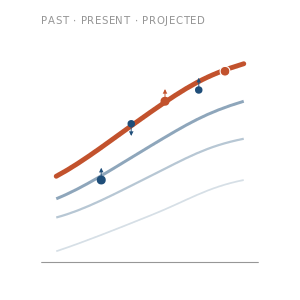
\includegraphics[height=6mm]{yc_logo.png}}
  \hfill{\ttfamily\scriptsize\color{ycmuted}yieldcartography.com/slides/liquidity/}
\end{frame}

\end{document}
